\documentclass{article}
\usepackage{graphicx} % Required for inserting images
\usepackage{hyperref}
\usepackage{tikz}
\usepackage{tabularray}
\usepackage{pgfplots}
\usepackage{float}
\usepackage{listings}
\title{Genetic Algorithm and Simulated Annealing solutions to TSP}
\author{Denis Crismariu}
\date{\today}



\usepackage{color}

\definecolor{dkgreen}{rgb}{0,0.6,0}
\definecolor{gray}{rgb}{0.5,0.5,0.5}
\definecolor{mauve}{rgb}{0.58,0,0.82}

\lstset{frame=tb,
	language=Python,
	aboveskip=3mm,
	belowskip=3mm,
	showstringspaces=false,
	columns=flexible,
	basicstyle={\small\ttfamily},
	numbers=none,
	numberstyle=\tiny\color{gray},
	keywordstyle=\color{blue},
	commentstyle=\color{dkgreen},
	stringstyle=\color{mauve},
	breaklines=true,
	breakatwhitespace=true,
	tabsize=3,
}



\begin{document}

\maketitle

\abstract

This report investigates the application of Genetic Algorithms (GA) and Simulated Annealing (SA) for solving the Traveling Salesman Problem (TSP) on 10 sample datasets. The study focuses on the implementation and experimentation with different optimization techniques to enhance the performance of the GA and compares it with the SA. Through detailed experimentation, we evaluate the efficiency and accuracy of both algorithms on the TSP datasets. This report aims to provide insights into the effectiveness of various optimization strategies in genetic algorithms and suggests potential areas for further research and improvement. Our experiments show that for smaller samples, SA is much faster and provides similar results to the GA. However, for larger samples, the inaccuracy and time spent by SA grow exponentially. The findings highlight the trade-offs between accuracy and performance in optimization algorithms and offer guidance for selecting appropriate techniques for solving TSP and similar combinatorial problems.

\section{Introduction}
This report explores the use of Genetic Algorithms (GA) and Simulated Annealing (SA) for solving the Traveling Salesman Problem (TSP) on 10 sample datasets. The study focuses on implementing and experimenting with optimization techniques to enhance GA performance and compares it with SA. The objective is to find the optimal route that minimizes the total travel distance.

GA begins with an initial population of potential solutions, represented as permutations of cities, and evolves through fitness evaluation, selection, crossover, and mutation. SA starts with a single solution and iteratively improves it by exploring neighboring solutions, accepting worse solutions with a certain probability to escape local minima.

This report provides a detailed analysis of GA and SA performance on TSP datasets, highlighting the impact of different optimization strategies. By comparing GA with SA, we explore trade-offs and potential strategies for enhancing algorithm performance. Our experiments show that for smaller samples, SA is much faster and provides similar results to GA. However, for larger samples, SA's inaccuracy and time spent grow exponentially. The findings highlight the trade-offs between accuracy and performance in optimization algorithms and offer guidance for selecting appropriate techniques for solving TSP and similar combinatorial problems.



\section{Comparison in Pseudocode}

\begin{lstlisting}
# Genetic Algorithm
	for i in [0,greedy):
		pop[i]=greedy_init() # initialize using a greedy
	for i in [greedy,size):
		pop[i]=rand() # generate a random permutation
		
	for e in [1,epoch]:
		evaluation()
		copy_the_best(elit) # copy only top elit%
		for x in [1,size): 
			y1 = select()
			y2 = select()
			(pop[x],pop[x+1]) = crossover(y1,y2)
			mutate(x)
			mutate(x+1)
			
		if same_best > 50 : # we are stuck in a minima
			mut_rate = init_mut * 5 # mutation rate increases

# Simulated Annealing
	x = rand() # generate a random permutation
	path_max = min(5000,5*size)
	best_max = min(15000,50*size)
	while same_path < path_max and same_best < best_max:
		 n = rand_neighbor() # generate a random neighbor
		 if eval(n) better eval(x):
		 	x = n
		 else if rand[0,1) < exp(-|eval(x)-eval(n)|/T)
		 	x = n
	T*=alfa 
		 
\end{lstlisting}


\pagebreak
\section{Methods \& Implementation}

\subsection{Initialization}  
The Genetic Algorithm (GA) begins by generating an initial population of 200 individuals, each representing a possible solution to the Traveling Salesman Problem (TSP). The algorithm runs for a total of 3000 generations, ensuring sufficient time for refinement and convergence.  

The individuals are randomly generated, but to improve early convergence, 10\% of the population is initialized using a greedy heuristic. This heuristic starts from a randomly chosen city and iteratively adds the nearest unused city until a complete tour is formed. This ensures that part of the population consists of high-quality solutions from the beginning, accelerating the optimization process.  

\subsection{Fitness Evaluation}
The fitness of each individual is evaluated based on the total travel distance of its tour. Since the goal is to minimize the path length, we define the fitness function as $\frac{1}{f}$, ensuring that shorter paths have higher fitness values. This transformation makes selection more effective, as the best solutions naturally have higher probabilities of being chosen.

\subsection{Selection}
The selection process is based on the roulette wheel selection method, a probabilistic technique where individuals with higher fitness values have a greater chance of being selected. However, to maintain genetic diversity and prevent excessive self-replication, we ensure that both selected parents are distinct individuals. If the selection process chooses the same parent twice, a new second parent is chosen to guarantee diversity in crossover.

Additionally, elitism is applied, where the top 10\% of the best individuals are directly carried over to the next generation to ensure that the best solutions are preserved.

\subsection{Crossover}
For crossover, we use a modified Partially Mapped Crossover (PMX), ensuring that offspring inherit valid tour sequences from both parents. Unlike traditional PMX, this implementation mutates two paths simultaneously, increasing diversity and preventing premature convergence. This method effectively transfers genetic material while maintaining valid TSP paths.

\subsection{Mutation}  
Mutation introduces controlled randomness to explore new solutions and prevent premature convergence. Each individual (except the best from the last generation) undergoes one of the following two mutation types:  

\begin{itemize}  
	\item \textbf{Rotation Mutation} – A randomly selected segment of the tour is shifted to a new position.  
	\item \textbf{Inversion Mutation} – A randomly chosen segment of the tour is reversed in order.  
\end{itemize}  

To prevent stagnation, an adaptive mutation strategy is applied. If the best path remains unchanged for more than 50 generations, the mutation rate is increased fivefold, introducing greater variation and aiding in escaping local optima. Additionally, if the best path remains unchanged for 100 generations, the entire normal population (excluding elites) is shuffled, enforcing large-scale diversity in the population.  

Furthermore, after 100 generations of stagnation, a function is executed to compare the common edges among elite individuals. If two elite individuals share 100\% identical edges, one of them undergoes mutation to introduce variation while preserving high-quality solutions.  

These adaptive mechanisms ensure a balance between exploitation and exploration, preventing the algorithm from getting trapped in local minima while maintaining diversity among the best solutions.  

\subsection{Tour Encodings}  
In the process of implementing the Genetic Algorithm (GA) for the Traveling Salesman Problem (TSP), multiple encoding methods were explored to represent the tours efficiently. Two alternative encoding schemes were considered before settling on the permutation-based approach.  

\subsubsection{Inversion Sequence Encoding}  
The first approach follows the method proposed in \cite{ucoluk2002genetic}, where a permutation is described using its inversion sequence. For a permutation \(i_1, i_2, \dots, i_N\) of the set \(\{1, 2, \dots, N\}\), let \(a_j\) denote the number of integers in the permutation that precede \(j\) but are greater than \(j\). Thus, \(a_j\) measures how much out of order element \(j\) is. The sequence \(a_1, a_2, \dots, a_N\) is called the inversion sequence of the permutation.  

For example, the permutation:  
\[
4, 6, 2, 7, 3, 1, 5
\]  
has the inversion sequence:  
\[
5, 2, 3, 0, 2, 0, 0
\]  
Here, the 5th element in the inversion sequence is 2, meaning there are exactly two elements in the permutation that are to the left of 5 and are greater than 5 (which are 6 and 7).  

\subsubsection{Path-Based Index Encoding}  
The second encoding method represents a tour using a pathsize - 1 vector, where each position stores a random number between 0 and size()-1-position. This method ensures that each city is selected exactly once while maintaining a compact representation. The decoding process involves iterating through the sequence while keeping track of previously assigned cities.

For example, given the encoding:  
\[
\{0,2,1,2,1\}
\]  
the corresponding permutation (decoded path) would be:  
\[
\{0,3,2,5,4,1\}
\]  
where each number in the encoded sequence determines the position of the next available city in the ordering process.

\subsubsection{Final Choice: Permutation-Based Encoding}  
Although these alternative encoding methods provided compact representations of tours, they did not yield sufficiently strong results. The additional complexity of decoding and optimizing these encodings made it difficult to fine-tune the genetic algorithm efficiently.  

Due to these limitations, the permutation-based approach was ultimately chosen. While it sacrifices some encoding efficiency, it offers better optimization potential, ease of use, and stronger performance. Additionally, the extensive documentation and available research on optimizing permutation-based genetic algorithms further justified this decision.  




\section{Experimental results}
\begin{table}[!h]
	\centering
	\begin{tblr}{
			width = \linewidth,
			colspec = {Q[162]Q[152]Q[152]Q[152]Q[179]Q[135]},
			row{1} = {c},
			column{even} = {r},
			column{3} = {r},
			column{5} = {r},
			cell{1}{1} = {c=6}{0.931\linewidth},
			cell{2}{2} = {c},
			cell{2}{3} = {c},
			cell{2}{4} = {c},
			cell{2}{5} = {c},
			cell{2}{6} = {c},
			hlines,
			vlines,
		}
		GA        &          &          &          &            &          \\
		Instance  & Expected & Best     & Mean     & StDev      & Error    \\
		berlin52  & 7542     & 7542     & 7542     & 87.533     & 0.000\%  \\
		st70      & 675      & 675      & 685      & 3.758      & 0.000\%  \\
		rat99     & 1211     & 1211     & 1245     & 15.597     & 0.000\%  \\
		pr124     & 59030    & 59246    & 59889    & 680.858    & 0.366\%  \\
		bier127   & 118282   & 118728   & 119904   & 986.905    & 0.377\%  \\
		ch130     & 6110     & 6162     & 6370     & 123.507    & 0.851\%  \\
		a280      & 2579     & 2584     & 2637     & 34.908     & 0.194\%  \\
		brd14051  & 469385   & 570121   & 572480   & 1119.781   & 21.461\% \\
		d18512    & 645238   & 783126   & 786156   & 1259.225   & 21.370\% \\
		pla338110 & 66048945 & 77187360 & 77711136 & 185961.500 & 16.864\% 
	\end{tblr}
\end{table}
\pagebreak
\begin{table} [!h]
	\centering
	\begin{tblr}{
			width = \linewidth,
		colspec = {Q[162]Q[152]Q[152]Q[152]Q[179]Q[135]},
		row{1} = {c},
		column{even} = {r},
		column{3} = {r},
		column{5} = {r},
		cell{1}{1} = {c=6}{0.931\linewidth},
		cell{2}{2} = {c},
		cell{2}{3} = {c},
		cell{2}{4} = {c},
		cell{2}{5} = {c},
		cell{2}{6} = {c},
		hlines,
		vlines,
		}
		SA        &          &         &         &            &         \\
		Instance  & Expected & Best    & Mean    & StDev      & Error   \\
		berlin52  & 7542     & 7542    & 7914    & 294.055    & 0.000\%   \\
		st70      & 675      & 675     & 697     & 18.939     & 0.000\%   \\
		rat99     & 1211     & 1213    & 1289    & 26.121     & 0.165\%   \\
		pr124     & 59030    & 59030   & 61314   & 2299.132   & 0.000\%   \\
		bier127   & 118282   & 118725  & 126235  & 3422.159   & 0.375\%   \\
		ch130     & 6110     & 6174    & 6507    & 157.911    & 1.047\%   \\
		a280      & 2579     & 2661    & 2868    & 63.056     & 3.180\%   \\
		brd14051  & 469385   & 1654292 & 1877874 & 172586.600 & 252.438\% \\
		d18512    & 645238   & 2634013 & 2898515 & 234024.000 & 308.223\% \\
		pla338110 & 66048945 & N/A     & N/A     & N/A        & N/A       
	\end{tblr}
\end{table}

 I was unable to get a single simulated annealing (SA) run to finish the problem pla338110 within the time limit, even after running the code for 3 days. I did not want to lower the halting criteria for the SA, as the error was already too large with the current settings. \\
To estimate the time required for completion, I used Desmos for linear regression, which gave an estimate of an average of 33,696 seconds per sample, which translates to approximately 12 days of computation.


\begin{figure}[H]%means place figure here, don't float it around, if possible
	\centering %inside a figure, centers the content
	\begin{tikzpicture}
		\begin{axis}[
			height=0.6\textheight, % Set the height of the plot
			width=\textwidth, % Set the width of the plot
			xlabel=dimensions,
			ylabel=mean time,
			legend pos=north west,
			]		
			
			\addplot [
			color=blue,
			domain=52:338110, % Set the range of x-values for the plot
			]
			{0.0997217*x-20.75007}; % The function you obtained from Desmos
			\addlegendentry{SA Fitted Curve}
			
			\addplot [
			color=red, 
			]
			coordinates {
				(52,0.012)
				(70,0.024)
				(99,0.053)
				(124,0.100)
				(127,0.105)
				(130,0.114)
				(280,0.905)
				(14051,1138.173)
				(18512,2008.954)
				
			};
			\addlegendentry{SA}
			
			
			\addplot [
			color=green, 
			]
			coordinates {
				(52,1.755)
				(70,2.242)
				(99,3.413)
				(124,1.209)
				(127,10.412)
				(130,11.095)
				(280,54.748)
				(14051,126.962)
				(18512,160.163)
				(338110,451.327)
				
			};
			\addlegendentry{GA}
			
			\addplot[only marks, mark=*, color=purple] coordinates {(338110,33696.13787)};
			\node at (axis cs:338110,33696.13787) [anchor=south east] {$(338110, 33696.13787)$}; % Label the point
			
			\addplot[only marks, mark=*, color=purple] coordinates {(18512,2008.954)};
			\node at (axis cs:18512,2008.954) [anchor=south west] {$(18512,2008.954)$}; % Label the 
			
			\addplot[only marks, mark=*, color=purple] coordinates {(338110,451.327)};
			\node at (axis cs:338110,451.327) [anchor=south east] {$(338110, 451.327)$}; % Label the point
			
		\end{axis}
	\end{tikzpicture}
\end{figure}


\section{Comparing Methods}

While simulated annealing (SA) has proven to be faster and more accurate on small sample sizes, its performance degrades significantly when applied to larger datasets. In smaller samples, the method offers higher accuracy and reduced computation time. However, as the sample size increases, both the error and the runtime grow exponentially. For example, on the second-largest sample, the error from simulated annealing was 3.5 times larger than that of the genetic algorithm (GA), and the time it took was 25 times longer. This exponential increase in error and time makes simulated annealing less efficient for larger datasets, where other optimization methods, such as the GA, may become more suitable due to their scalability and better performance under such conditions.


\section{Conclusion}

The Traveling Salesman Problem (TSP) remains a challenging problem, even for optimization techniques like genetic algorithms. While the genetic algorithm shows promise, there are still areas for improvement. For instance, combining the genetic algorithm with simulated annealing could enhance performance, as both methods have complementary strengths. Additionally, exploring different encoding strategies and fine-tuning parameters could yield further improvements, potentially making the algorithm more efficient and accurate for larger datasets. Ongoing research into hybrid approaches and optimization techniques is crucial for addressing the complexities of TSP and finding more effective solutions.



\begin{thebibliography}{9}


\bibitem{paper}
Üçoluk, Göktürk. "Genetic algorithm solution of the TSP avoiding special crossover and mutation." Intelligent Automation \& Soft Computing 8.3 (2002): 265-272.

\bibitem{samples}
TSP problems:\\
\url{http://comopt.ifi.uni-heidelberg.de/software/TSPLIB95/}

\bibitem{}
Laboratory site: \\
\url{https://profs.info.uaic.ro/~eugennc/teaching/ga/}


\bibitem{PMX}
PMX Crossover:\\ \href{https://itnext.io/the-genetic-algorithm-and-the-travelling-salesman-problem-tsp-31dfa57f3b62}
{https://itnext.io/the-genetic-algorithm-tsp}
\url{}
\bibitem{SA}
SA for TSP : \\ \href{https://medium.com/@francis.allanah/travelling-salesman-problem-using-simulated-annealing-f547a71ab3c6}
{https://medium.com/@francis.allanah/tsp-using-simulated-annealing}

\end{thebibliography} 

\end{document}




